\documentclass[a4paper,12pt]{article}
%\usepackage[catalan]{babel}
\usepackage[utf8]{inputenc}
\usepackage{amsfonts}
\usepackage[colorlinks=true]{hyperref}
\usepackage[left=2.5cm,right=2.5cm]{geometry}
\usepackage{graphicx}
\usepackage[labelformat=empty]{caption}
\usepackage[ngerman]{babel}
\usepackage{gensymb}

\hyphenation{al-ler-dings ein-zig-ar-ti-ge ge-ra-de ne-ben-ach-se Platt-kar-te
             Halb-ge-ra-de Halb-ach-sen}


\title{Karten der Erde \\ Aktivitäten}
\author{Daniel Ramos\footnote{E-mail: \texttt{daniel.ramos@mmaca.cat}}
        \\MMACA (Museu de Matemàtiques de Catalunya)
        \\übersetzt von Hannes Grimm--Strele\footnote{E-mail: \texttt{hannes.grimm-strele@gmx.net}}}

\date{\today}

\pagestyle{empty}

\begin{document}
\maketitle

\begin{abstract}
  In diesem Dokument sammeln wir Vorschläge, wie man mit den Werkzeugen, den Postern
  und der Software des Ausstellungsstücks "`Karten der Erde"' arbeiten kann. Für eine 
  Beschreibung der Werkzeuge verweisen wir auf das entsprechende Dokument.
  Dieses Dokument ist als Grundlage vorgesehen, von der ausgehend man entweder eine 
  Vorlesung vorbereiten kann, oder das man ausgedruckt neben den einzelnen Stationen
  aufhängt. Diese Unterlagen sind in einem vorläufigen 
  Zustand und noch nicht ausreichend getestet und überprüft. Daher können sie noch
  Tipp-- und andere Fehler enthalten. Bitte lies dieses Dokument gründlich, 
  bevor du "`Karten der Erde"' in einer öffentlichen Ausstellung verwendst, und 
  schreibe Probleme und Anregungen an den Autor.
\end{abstract}


Wir schlagen vor, das Dokument wie folgt zu verwenden: Abschnitt~\ref{sec-map} ist als
ein\-führ\-en\-des Material vorgesehen und sollte möglichst nahe beim Globus und den 
entsprechenden Materialien platziert werden. Die Abschnitte~\ref{sec-plate} 
bis~\ref{sec-mollweide} sollten direkt neben dem entsprechenden Poster aufgehängt 
werden. Der Abschnitt~\ref{sec-distortion} ist thematisch dem Computer zugeordnet und 
sollte gelesen werden, nachdem man die Poster betrachtet hat. Das in 
Abschnitt~\ref{sec-inside} gesammelte Material ist als Ergänzung für interessierte 
Besucher vorgesehen.



\newpage
\section{Was ist eine Kartenabbildung?}
\label{sec-map}

Eine \emph{Kartenabbildung} oder \emph{Projektion} ist eine flache Darstellung der 
Erdoberfläche. Als Karte bezeichnen wir das durch die Kartenabbildung erzeugte Bild 
der Erdoberfläche. Zwar gibt es unendlich viele solcher Abbildungen, jedoch verzerren 
alle die Darstellung in der einen oder anderen Weise. Abhängig von der beabsichtigten 
Nutzung der Karte möchten wir manche Eigenschaften der Erde in der Abbildung erhalten und 
müssen dafür den Verlust anderer Eigenschaften in Kauf nehmen. Beispielsweise ist es für 
Seekarten wichtig, den Winkel einer Route zum Nordpol wirklichkeitsgetreu darzustellen,
damit wir ihn mit dem Ausschlag der Kompassnadel vergleichen können. Wenn wir hingegen 
Klimazonen auf der Erde darstellen wollen, wäre es sehr viel nützlicher eine Karte 
zu verwenden, die Flächeninhalte nicht verzerrt.

\begin{itemize}
 \item Betrachte den Globus und einige wichtige Kartenabbildungen. Ähneln sie der 
       Erd\-ober\-fläche? Kannst du die Verzerrung durch die Abbildung beschreiben oder 
       sogar anhand der Eigenschaften der Abbildung erklären?
 \item Betrachte das Gitter auf dem Globus und auf den Karten. Wozu ist es da? Hilft es, 
       die Verzerrungen zu erkennen?
\end{itemize}

\subsection*{Koordinaten}

Das Koordinatensystem der Erde erlaubt, einen Punkt $p$ auf der Oberfläche mit Hilfe
zweier Zahlen zu identifizieren: \emph{Längengrad} ($\lambda$) und \emph{Breitengrad} 
($\phi$). Auf der Erdoberfläche gibt es feste Bezugspunkte: den Nord-- und den Südpol 
definiert durch die Erdachse, die Äquatorebene, die im rechten Winkel zur Erdachse steht 
und sie in ihrem Mittelpunkt schneidet, und die Halbebene, die das Greenwich Royal 
Observatory sowie die Erdache enthält. Der Längengrad ist der Winkel zwischen der Linie, 
die den Punkt $p$ mit dem Erdmittelpunkt verbindet, sowie der Äquatorebene.

\begin{itemize}
 \item Finde Längen-- und Breitengrad auf der durchsichtigen Halbkugel.
\end{itemize}

Ein \emph{Längenkreis} oder \emph{Meridian} ist eine Linie mit festem Längengrad, 
während man Linien, entlang derer der Breitengrad sich nicht ändert, \emph{Breitenkreise} 
nennt. Auf dem Globus sind Längen-- und Breitenkreise mit jeweils 10º Abstand 
eingezeichnet.

Auf dem Globus kann man Entfernungen zwischen zwei Punkten entweder in Kilometern oder 
über die Bogenlänge messen, wobei man den Erdmittelpunkt als weiteren Eckpunkt wählt.
Die Bogenlänge kann dann mittels der Formel Bogenlänge $= {\rm Winkel} \cdot  
{\rm Radius}$ berechnet werden.

\begin{itemize}
 \item Versuche, vom Globus und den Karten die Koordinaten einiger Städte abzulesen.
 \item Verwende das biegbare Lineal, um einige Entfernungen zu messen. Beachte dabei,
       dass das Lineal zwei Skalen besitzt: eine in Kilometern und eine in Grad.
\end{itemize}





\newpage
\section{Die Plattkarte}
\label{sec-plate}
Die Plattkarte ist die wahrscheinlich einfachste Kartenabbildung. Längen-- und 
Breitengrad werden dabei als $x$-- und $y$--Koordinate in der Ebene gewählt. 
Daher ist das Gitter auf der Plattkarte quadratisch und die Gitterlinien haben 
gleichen Abstand. Ist diese Abbildung wirklichkeitsgetreu?

\begin{itemize}
 \item Jedes Quadrat auf der Plattkarte entspricht auf der Erdoberfläche einem Gebiet, 
       dass 10º Differenz in Längen-- und Breitengrad umfasst. Ist jedoch das Gitter 
       auf der Erdoberfläche quadratförmig? Überprüfe die Seitenlänge eines "`Quadrates"'
       nahe beim Äquator und nahe der Pole. Sind die Seiten gleich lang? Wie lange ist 
       ein Bogen von 10º in einem Breitenkreis nahe beim Äquator, und wie lange bei 
       70º nördlicher Breite?
 \item Können wir das Maßband auf dieser Karte verwenden?
\end{itemize}

Um näher an der Wirklichkeit zu sein, sollte die Projektion des Gitters auf die Karte 
daher nicht quadratisch sein.



 
\newpage
\section{Die Mercator--Projektion}
\label{sec-mercator}

Diese Abbildung wurde 1569 von Gerardus Mercator erfunden und ist zweifellos die 
historisch gesehen wichtigste Kartenabbildung. Diese Abbildung wird oft standardmäßig 
für die Darstellung der Erdoberfläche verwendet. Betrachten wir ein "`Gitterquadrat"' 
nahe bei den Polen, stellen wir fest, dass diese eher die Form von Rechtecken haben. 
Die Mercator--Projektion ist eine vertikale Verzerrung der Plattkarte. Da die 
Breitenkreise länger zu sein scheinen als sie tatsächlich sind, werden sie
im gleichen Maß gestreckt, so dass die Karte vertikal und horizontal in jedem Punkt 
gleichermaßen gestreckt ist. Flächen werden dabei stark verzerrt, dafür hat diese 
Abbildung eine andere wichtige Eigenschaft: Form und Winkel bleiben erhalten.

Für die Navigation ist Folgendes von zentraler Bedeutung. Wenn man mit dem Schiff von 
einer Stadt zu einer anderen segeln will und eine gerade Verbindungslinie auf einer 
von der Mercator--Projektion erzeugten Karte einzeichnet, schneidet diese Linie, 
\emph{Loxodrome} genannt, die vertikalen Längenkreise in einem konstanten, nach Norden 
zeigenden Winkel. Da Winkel durch die Abbildung erhalten werden, ist dieser Schnittwinkel 
genau der Winkel, der auf dem Kompass eingestellt werden muss, um zum Ziel zu kommen
(abgesehen von dem kleinen Fehler durch den Unterschied zwischen magnetischem und 
geografischem Nordpol). Auf diese Art und Weise kann und konnte man jahrhundertelang 
einen "`Kurs"' festlegen, um von einem Ort zu dem anderen zu navigieren. Allerdings ist 
die Loxodrome nicht die kürzeste Verbindung!

\begin{itemize}
 \item Stelle dir vor, du wärst im 16.\ Jahrhundert und möchtest von Cadiz im Süden 
       von Spanien nach Caracas in Venezuela mit deiner Karavelle segeln. Welche 
       Route ist am einfachsten für die Navigation? Verwende dazu den Winkelmesser 
       für die Ebene.

 \item Stelle dir vor, du willst heutzutage von Athen in Griechenland nach Los Angeles 
       in den USA fliegen. Wo verläuft die Loxodrome, die diese Städte verbindet?

       In Wirklichkeit würdest das Flugzeug jedoch über Grönland fliegen. Warum? 
       Suche auf dem Globus die kürzeste Strecke.

 \item Überprüfe mit den zwei Winkelmessern, dass die Winkel entlang der Loxodrome 
       auf der Karte und auf dem Globus gleich sind.
\end{itemize}



\newpage
\section{Die Gall--Peters--Projektion}
\label{sec-gall}

Die Mercator--Projektion hat im Vergleich zur Plattkarte den Vorteil, dass sie die 
Winkel erhält. Dafür verzerrt sie aber Flächen stark. Andere Kartenabbildungen wie die
Gall--Peters--Projektion erhalten Flächen. Man nennt diese Abbildung auch die 
"`Dritte Welt--Karte"', da Länder in Afrika und Südamerika sowie alle Gegenden nahe 
beim Äquator auf der Karte hervorstechen. Afrika ist auf der Karte größer als Europa,
entsprechend den realen Größenverhältnissen. Dafür wird die Form nicht erhalten: Afrika
ist nicht so schmal wie es auf der Karte zu sein scheint.

\begin{itemize}
 \item Ist Nordamerika größer als Afrika oder umgekehrt? Beantworte diese Frage mit 
       Hilfe der Gall--Peters--Projektion. Wie ist das Größenverhältnis unter der 
       Mercator--Projektion?
       (Die Fläche Nordamerikas ist etwa $24\,709\,000\,{\rm km}^2$, die Fläche 
       Afrikas etwa $30\,221\,532\,{\rm km}^2$.)

 \item Vergleiche die Form und die Größe der Kontinente mittels der Schablonen 
       auf der Karte und auf dem Globus. Passen sie zusammen? Was passiert mit der 
       Antarktis?
\end{itemize}



\newpage
\section{Die mittabstandstreue Azimutalprojektion}
\label{sec-azimuthal}

Diese Projektion nennt man auch "`Flughafen--Abbildung"'. In der aktuellen Einstellung 
ist Barcelona als Zentrum der Karte gewählt, aber diese Wahl ist beliebig und kann 
durch jeden anderen Ort ersetzt werden. Nachdem wir das Zentrum gewählt haben, zeichnen
wir alle Punkte gleichen Abstands vom Zentrum auf konzentrische Kreise um das Zentrum,
indem wir die Entfernung als Radius wählen. Daher wird auf der Karte die Entfernung 
jedes Punktes zu Barcelona korrekt dargestellt (alle anderen Entfernungen sind allerdings 
verzerrt!). Der Winkel zwischen der Verbindungslinie zwischen Barcelona und dem Zielpunkt 
und der vertikalen Richtung nach Norden ist ebenfalls korrekt. Daher ist diese Karte 
am Flughafen von Barcelona sehr nützlich, da man einfach erkennen kann, wie weit 
entfernt das Ziel ist und über welche Länder man fliegen wird. Man kann damit auch 
die Entfernungen verschiedener Städte von Barcelona vergleichen.

Wir können das Maßband nur dazu verwenden, Entfernungen von Barcelona aus zu messen;
für alle anderen Strecken wird die gemessene Entfernung falsch sein.

\begin{itemize}
 \item Wie weit sind New York (USA), Kapstadt (Südafrika) und Tokio (Japan) von 
       Barcelona entfernt?
 \item Was ist der Durchmesser dieser Karte?
 \item Wie viele Länder kannst du von Barcelona aus besuchen, wenn du weniger als 
       $10\,000\,{\rm km}$ reist?
 \item Als Antipode bezeichnet man den Punkt, der sich auf der gegenüberliegenden
       Seite der Erdkugel befindet. Die Antipode von Barcelona befindet sich irgendwo 
       im Pazifischen Ozean nahe bei Neuseeland. Findest du diesen Punkt auf der Karte?
       Wo ist Neuseeland?
\end{itemize}



\newpage
\section{Die gnomonische Projektion}
\label{sec-gnomic}

Die mit dieser Projektion erzeugte Karte wirkt stark verzerrt. Dennoch hat sie eine 
einzigartige Eigenschaft: die kürzeste Verbindungslinie zweier Punkte, auch Geodäte 
genannt, wird als gerade Linie dargestellt. Das bedeutet, dass du, wenn du die 
Verbindungslinie als gerade Linie darstellen willst, die Karte entsprechend verzerren 
musst. Auf dieser Karte kann man nicht die gesamte Erdoberfläche darstellen, sondern nur 
einen Teil, der kleiner ist als die Hälfte. Wir haben wieder Barcelona als Zentrum 
gewählt. Du erhältst diese Karte, indem du jeden Punkt auf der Erdoberfläche durch das 
Erdzentrum auf eine Tangentialebene mit Barcelona als Zentrum projizierst.

\begin{itemize}
 \item Finde die kürzeste Verbindung von Jerusalem (Israel) nach Havanna (Kuba). 
       Über\-quert die Linie Afrika? Hättest du das auch gedacht, wenn du die anderen 
       Karten betrachtest?
 \item Welche Form nehmen Längen-- und Breitenkreise an?
\end{itemize}





\newpage
\section{Die Mollweide--Projektion}
\label{sec-mollweide}

Die von dieser Projektion erzeugte Karte füllt eine Ellipse aus, die doppelt so 
lang wie hoch ist. Sie löst ein Problem, das viele zylindrische Projektionen wie 
die Plattkarte, die Mercator--, die Gall--Peters-- und einige anderen Projektionen 
haben. In der Mollweide--Projektion werden die Pole an eindeutigen Punkten angezeigt,
während sie z.B. auf der Plattkarte den oberen und unteren Rändern der Karte 
entsprechen. Dadurch werden die Gegenden um die Pole, also Arktis und Antarktis, 
extrem verzerrt. Die Mollweide--Projektion hat dieses Problem nicht und reduziert 
daher die Verzerrungen beträchtlich. Außerdem erhält sie den Flächeninhalt. Wegen 
ihrer gebogenen Ränder erinnert ihr Umriss an den Umriss der Erdkugel.

\begin{itemize}
 \item Wie werden Längen-- und Breitenkreise dargestellt?
 \item Vergleiche diese Projektion mit der Gall--Peters--Projektion. Beide erhalten 
       den Flächeninhalt. Welche verzerrt deiner Meinung nach die Erde weniger?
       Verwende die Schablonen der Kontinente auf beiden Abbildungen und dem Globus.
\end{itemize}



\newpage
\section{Können wir die Verzerrung messen?}
\label{sec-distortion}

Die Verzerrung einer Kartenabbildung ist eine schwierig zu messende Größe und kaum 
durch eine einzelne Maßzahl auszudrücken. Stattdessen hat der französische Mathematiker
Nicolas Auguste Tissot 1859 eine grafische Methode entwickelt, um die Verzerrung in 
einem Punkt auf der Karte darzustellen. Stell dir einen kleinen Kreis um einen beliebigen 
Punkt auf der Erdoberfläche vor. Nach der Projektion auf die Karte wird dieser Kreis 
durch die Verzerrung nicht mehr kreisförmig sein. Wenn der Kreis klein genug ist, wird
er auf eine Ellipse projiziert werden -- mathematisch gesehen aber erst für verschwindend 
kleinen Radius, wie in Abbildung~\ref{tiss_diagram} dargestellt. Wir vergrößern 
diese Ellipse so lange, bis wir sie auf der Karte sehen können. Wir nennen sie die 
\emph{Tissotsche Indikatrix} der Karte, und können mit ihrer Hilfe viele Informationen 
über die Verzerrungen durch die Projektion herausfinden.

\begin{figure}[h]
 \begin{center}
  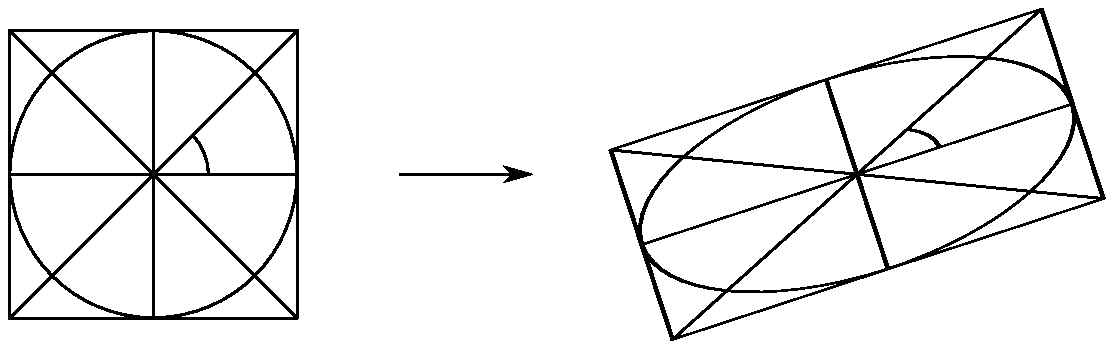
\includegraphics[width=0.7\textwidth]{../common/tiss_diagram} 
\caption{Ein Kreis mit verschwindendem Radius wird auf eine Ellipse projiziert.}
\label{tiss_diagram}
 \end{center}
\end{figure}

\begin{itemize}
 \item Betrachte die Ausgabe des Programms auf deinem Bildschirm. Mit den Registerkarten
       in der Leiste am oberen Rand kannst du eine Abbildung auswählen. Wenn du den
       Mauszeiger über die Karte bewegst, erscheint die Tissotsche Ellipse für den
       entsprechenden Punkt. Wenn du auf die Karte klickst, bleibt die Ellipse an 
       diesem Punkt fixiert. Im rechten unteren Eck kannst du die Größe der Ellipse
       verändern und alle angezeigten Ellipsen entfernen.
\end{itemize}


\paragraph{Die Hauptrichtungen.}
Indem die Projektion die Karte staucht und streckt, entsteht eine Verzerrung. Je nach 
Projektion kann die Verzerrung die Karte in die eine Richtung stauchen und in die andere 
Richtung strecken, je nach Punkt, an dem wir uns befinden. Die zwei Achsen der Tissotschen
Ellipse zeigen die \emph{Hauptrichtungen} an. Das sind die Richtungen, in denen 
die Karte am stärksten und am schwächsten gestreckt wird. Wenn die Ellipse extrem  
abgeplattet ist, d.h.\ wenn ihre Hauptachse sehr viel länger als ihre Nebenachse ist,
dann bedeutet das, dass die Verzerrung je nach Richtung sehr unterschiedlich wirkt.

\begin{itemize}
 \item Unter welchen Projektionen sind die Ellipsen am stärksten verformt? Welche Form 
       haben die Ellipsen?
 \item Welche Form hat die Ellipse am Nordpol für die Plattkarte? Wo ist der Nordpol?
 \item Sind die Hauptrichtungen immer entlang der Längen-- und Breitenkreise?
\end{itemize}



\paragraph{Winkeltreue.} 
Wenn Haupt-- und Nebenachse der Tissotschen Ellipse gleich lang sind, wird die Ellipse 
zu einem Kreis und die Verzerrung ist in diesem Punkt in jede Richtung gleich stark.
Daher wird jede Form, wie z.B.\ eine Küstenlinie, in der Umgebung dieses Punktes in 
alle Richtungen gleichmäßig gestreckt, ohne verzerrt zu werden. Eine Projektion, die 
in keinem Punkt Formen verzerrt, wird \emph{winkeltreu} genannt. Aus 
Abbildung~\ref{tiss_diagram} folgern wir, dass alle Winkel durch die Projektion 
unverändert bleiben, wenn die Tissotsche Ellipse ein Kreis ist.
\emph{Winkeltreue Abbildungen lassen Winkel unverändert.}

\begin{itemize}
 \item Wenn die Tissotsche Ellipse zu einem Kreis wird, wird ihr Rand grün gefärbt.
       Finde für jede Karte die Punkte, wo die entsprechende Projektion winkeltreu 
       ist.
 \item Was ist an der Mercator--Projektion anders? Wie stark werden Winkel und Flächen 
       verzerrt?
\end{itemize}

\paragraph{Flächentreue.} 
Aus dem Flächeninhalt einer Ellipse können wir schließen, ob die Projektion 
in diesem Punkt im Mittel staucht oder streckt. Wenn ein kleiner Kreis mit Radius $r$ 
und Flächeninhalt $\pi r^2$ auf die Ellipse mit Haupt-- und Nebenachse
$a$ und $b$ projiziert wird und $a\,b = r^2$ gilt, bedeutet das, dass die Ellipse 
den gleichen Flächeninhalt wie der Kreis hat. Daraus folgt, dass die Abbildung den 
Flächeninhalt in diesem Punkt nicht verändert. 

Eine Abbildung, die Flächeninhalte erhält, wird \emph{flächentreue Projektion} genannt.

Wenn ein Punkt unter einer Projektion sowohl winkel-- als auch flächentreu ist, sagen 
wir, dass die Projektion in diesem Punkt \emph{maßstabsgetreu} ist. Dieser Punkt wird
auf der Karte ohne jede Verzerrung dargestellt. Ein wichtiger Satz aus der Geometrie
besagt, dass es keine Abbildung gibt, die alle Punkte maßstabsgetreu darstellen kann. 
Mit anderen Worten, es gibt keine "`perfekte"' Karte, die die gesamte Erdoberfläche 
maßstabsgetreu darstellt.

\begin{itemize}
 \item Wenn der Flächeninhalt durch die Projektion nicht verändert wird, wird das 
       Innere der Ellipse grün angezeigt. Welche Projektionen sind flächentreu? Was 
       ist der Flächeninhalt der gesamten Karte für diese Projektionen? 
 \item Vergleichen wir einmal den Flächeninhalt von Afrika und Grönland, zunächst unter 
       der Gall--Peters--Projektion. Wähle eine mittlere oder kleine Größe für die 
       Ellipsen aus. Wie viele kannst du auf Grönland platzieren, ohne dass sie sich 
       überschneiden? Und wie viele auf Afrika? Wiederhole dies für die 
       Mercator--Projektion. Wir erinnern uns: die Tissotschen Ellipsen sehen 
       unterschiedlich aus, \emph{stellen aber immer den gleichen Kreis auf der Erde 
       dar.}

       Je kleiner die Ellipse ist, die du auswählst, umso genauer wird die Näherung für 
       den Flächeninhalt. In Wirklichkeit ist Afrika $14{,}2$ mal so groß wie Grönland.
       Auf welchen zwei Karten wird dieses Größenverhältnis richtig dargestellt?
 \item Was ist größer: Grönland oder Australien? Was würdest du sagen, wenn du die 
       Plattkarte anschaust? Was erhältst du, wenn du die Tissotschen Ellipsen 
       verwendest?
 \item Sowohl die Gall--Peters-- als auch die Mollweide--Projektion sind flächentreu.
       Welche der beiden verzerrt Formen und Umrisse weniger stark?
 \end{itemize}



\begin{figure}[ht]
 \begin{center}
  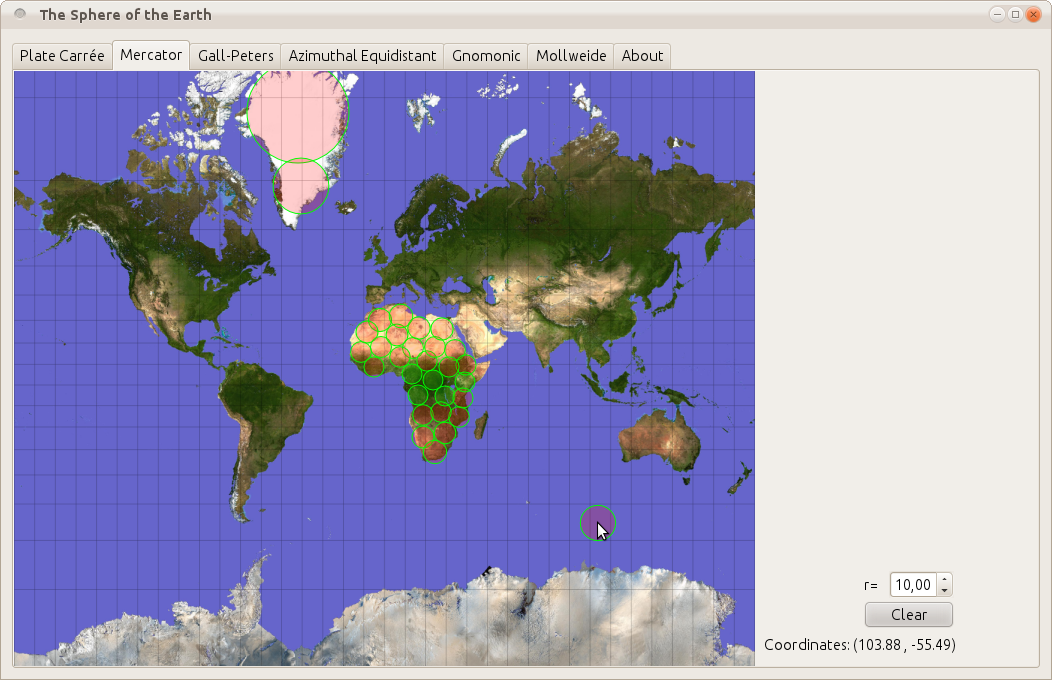
\includegraphics[width=0.7\textwidth]{../common/merc1.png} 
  \caption{Vergleich des Flächeninhalts von Afrika und Grönland unter der 
           Mercator--Projektion.}
 \end{center}
\end{figure}




\newpage
\section{Die Mathematik dahinter}
\label{sec-inside}

\textsf{In diesem Abschnitt geht es um höhere Mathematik. Lesen auf eigene Gefahr!}\\

Eine Kartenabbildung oder Projektion ordnet jedem Koordinatenpaar auf der Kugel 
$\mathbb S$ ein Koordinatenpaar auf der Ebene $\mathbb R^2$ zu,

$$\begin{array}{rccc}
   F: &\mathbb S & \longrightarrow & \mathbb R^2 \\
  & (\lambda, \phi) & \mapsto & (x,y),
  \end{array}
$$

\noindent wobei wir mit $\lambda$ den Längengrad und mit $\phi$ den Breitengrad 
bezeichnen. Diese Abbildung kann im Punkt $p$ durch die Tangentialabbildung $dF$

$$\begin{array}{rccc}
   dF_p: & T_p \mathbb S & \longrightarrow & \mathbb R^2 
  \end{array}
$$

\noindent beschrieben werden. Sie ordnet der Tangentialebene zur Kugel $\mathbb S$ im 
Punkt $p$ die Ebene $\mathbb R^2$ mit Zentrum $F(p)$ zu. Die Tangentialebene enthält 
also alle vom Punkt $p$ ausgehenden Richtungen. In diesem Sinne beschreibt der 
Einheitskreis alle Richtungsvektoren mit Länge $1$ in der Tangentialebene. Die Tissotsche 
Ellipse ist das Bild des Einheitskreises in der Tangentialebene $T_p \mathbb S$ unter der 
Abbildung $dF$. Wir können daher die Tissotsche Ellipse als Darstellung der Verzerrung 
der von $p$ ausgehenden Richtungsvektoren verstehen.

\begin{figure}[h]
 \begin{center}
  \def\svgwidth{ 0.85 \textwidth}
\input{../common/df.pdf_tex}
\caption{Die Abbildung $F$ und ihre Tangentialabbildung $dF$.}
 \end{center}
\end{figure}

Zwei Richtungen stehen sowohl auf die Erdoberfläche als auch auf die Karte senkrecht.
Um das zu sehen, betrachten wir eine beliebige Gerade $rs$ durch $p$ in der 
Tangentialebene und eine 
Halbgerade $t$, die in $p$ beginnt und im rechten Winkel auf $rs$ steht. Ihre Bilder 
$r's'$ und $t'$ berühren $p'=F(p)$, müssen aber nicht mehr im rechten Winkel zueinander 
stehen. Nehmen wir an, dass $r'p't'$ ein scharf-- und $t'p's'$ ein stumpfwinkliges 
Dreieck ist. Stellen wir uns vor, dass wir den rechten Winkel $rpt$ um $p$ rotieren,
bis wir auf dem Winkel $tps$ liegen. Auf der Karte beginnen wir mit dem spitzen Winkel 
$r'p't'$ und hören mit dem stumpfen Winkel $t'p's'$ auf. Also muss es dazwischen 
einen Punkt gegeben haben, wo der Winkel auf der Karte rechtwinklig war.

\begin{figure}[ht]
 \begin{center}
  \def\svgwidth{ 0.85 \textwidth}
\input{../common/diagonalize.pdf_tex}
\caption{Die Hauptrichtungen stehen im rechten Winkel zueinander.}
 \end{center}
\end{figure}

Diese zwei Richtungen sind die so genannten Hauptrichtungen. Sie werden durch 
zwei Einheitsvektoren beschrieben, die senkrecht zueinander stehen. Auf der Karte 
sind die Hauptrichtungen durch das Bild dieser zwei Vektoren gegeben und ihre Längen
$a$ und $b$ sind die Längen der Halbachsen der Tissotschen Ellipse. Im Fall $a=b$, wenn 
die Ellipse zum Kreis wird, sind alle Richtungen gleichermaßen verzerrt. Die 
Abbildung ist in diesem Punkt winkeltreu. Im Fall $a\,b=1$ hat die Ellipse den gleichen 
Flächeninhalt wie der Einheitskreis in der Tangentialebene. Mit einem unendlich 
großen Kreis erhalten wir die Oberfläche der Kugel. Daher ist die Abbildung in diesem 
Punkt flächentreu.

Formal gesprochen gilt, dass die Tangentialabbildung $dF$ diagonalisierbar in der 
Kugelmetrik ist, sowie dass die Eigenvektoren die Hauptrichtungen und die Eigenwerte 
die Halbachsen der Tissotschen Ellipse sind. Die Abbildung ist winkeltreu, wenn 
$dF$ ein Vielfaches der Einheitsmatrix ist, und flächentreu, denn $\det(dF)=1$.
Wenn beide Bedingungen in jedem Punkt erfüllt sind, ist $F$ eine Isometrie. Für 
den Fall der Erdoberfläche ist das auf Grund des Theorema egregium von Gauss 
nicht erfüllbar.
 
\end{document}

